% !TEX root = ../../技术文档.tex
\section{系统互连与存储仿真验证}

本节记录底层控制和互连的组件配置验证，其中CPU到NPU采用单算子MMIO，CPU到Video采用三路采集配置。本次头像应用整机的整帧图执行、两路采集及应用循环另见附录\ref{sec:box-system-validation}。
测试台均在Windows原生ModelSim中运行，图中波形为已保存WLF的原始Wave窗口截图。结果索引和源文件哈希见\path{docs/verification/soc/system_interconnect_storage_20261030.json}。

\subsection{CPU主端控制与外设访问}

CPU到Video的固件测试覆盖6个正例和2个负例。正例检查控制请求握手、三路AXI写通道、独立写响应、响应排空、完成事件和中断；负例分别注入错误响应和提前完成条件，均被测试台拒绝。图\ref{fig:system-interconnect-cpu-video}给出一组原始仿真波形：请求握手后，AW/W/B通道交错推进，\texttt{port\_drained}保持为零直到写响应全部排空，随后才产生\texttt{completion\_valid}和中断。

\begin{figure}[!htbp]
\centering
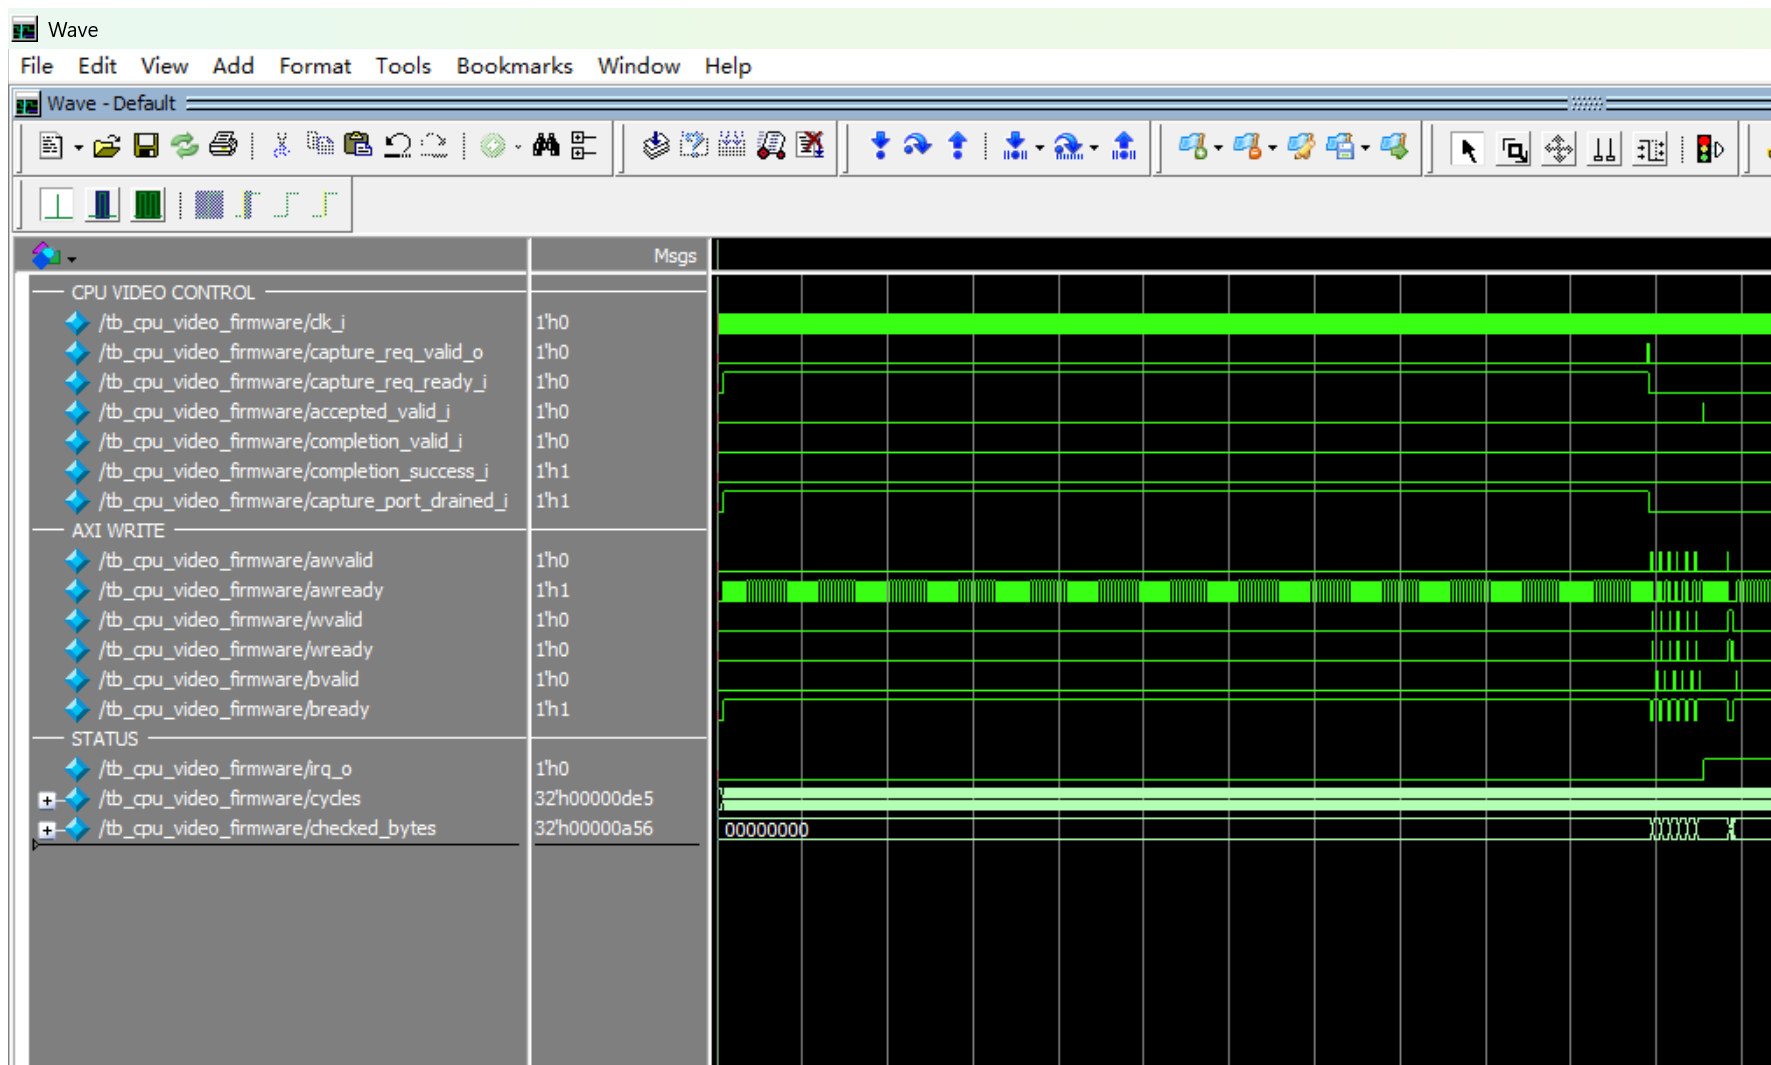
\includegraphics[width=0.8\linewidth]{../figure/system-interconnect-cpu-video-modelsim-original.png}
\caption{CPU到Video控制请求、AXI写入、响应排空和完成中断波形}
\label{fig:system-interconnect-cpu-video}
\end{figure}

CPU到NPU的算子测试覆盖Dense U8和DW S8两类算子，分别检查轮询和中断完成路径，共4个正例通过。图\ref{fig:system-interconnect-cpu-npu-control}展示AXI-Lite参数写入与AXI128读写启动阶段，图\ref{fig:system-interconnect-cpu-npu-complete}展示尾部写响应、读写握手背压以及事务计数收敛；\texttt{DONE}只在最后一个写响应完成后产生。

\begin{figure}[!htbp]
\centering
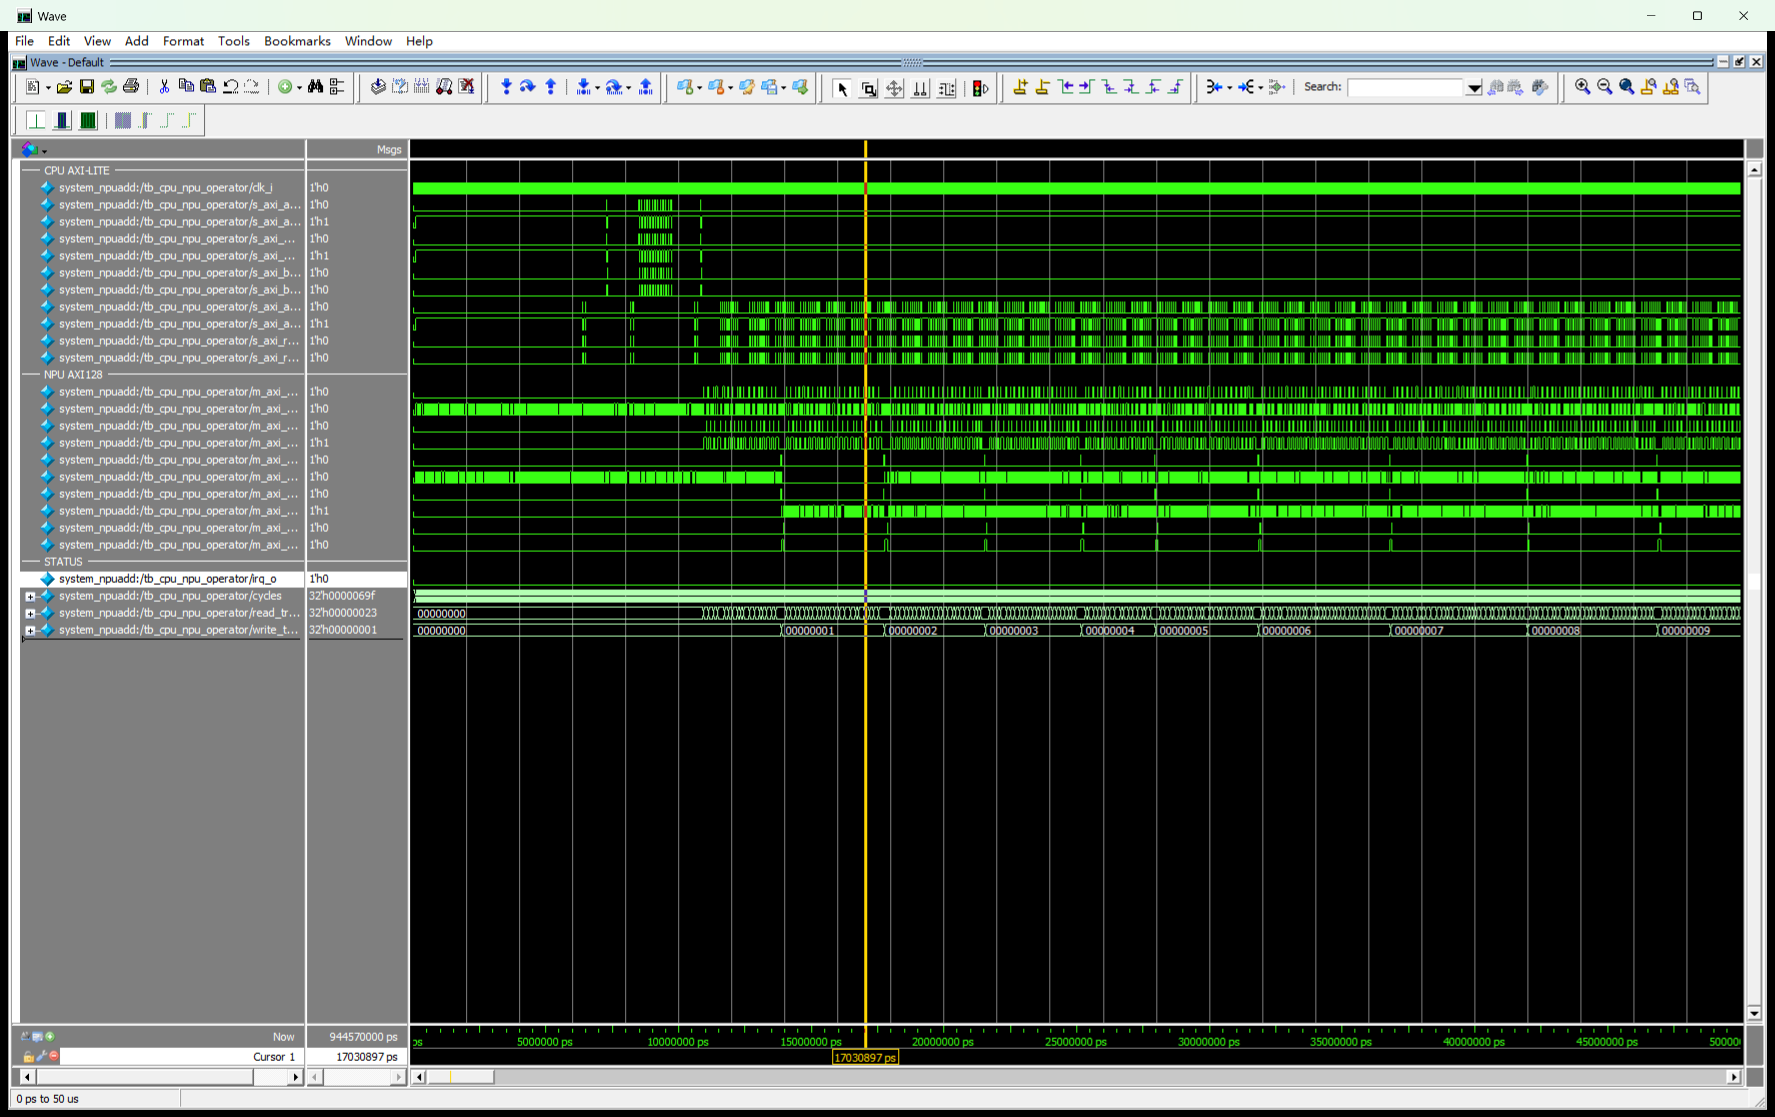
\includegraphics[width=0.8\linewidth]{../figure/system-interconnect-cpu-npu-control-modelsim-original.png}
\caption{CPU到NPU的AXI-Lite配置与AXI128初始传输波形}
\label{fig:system-interconnect-cpu-npu-control}
\end{figure}

\begin{figure}[!htbp]
\centering
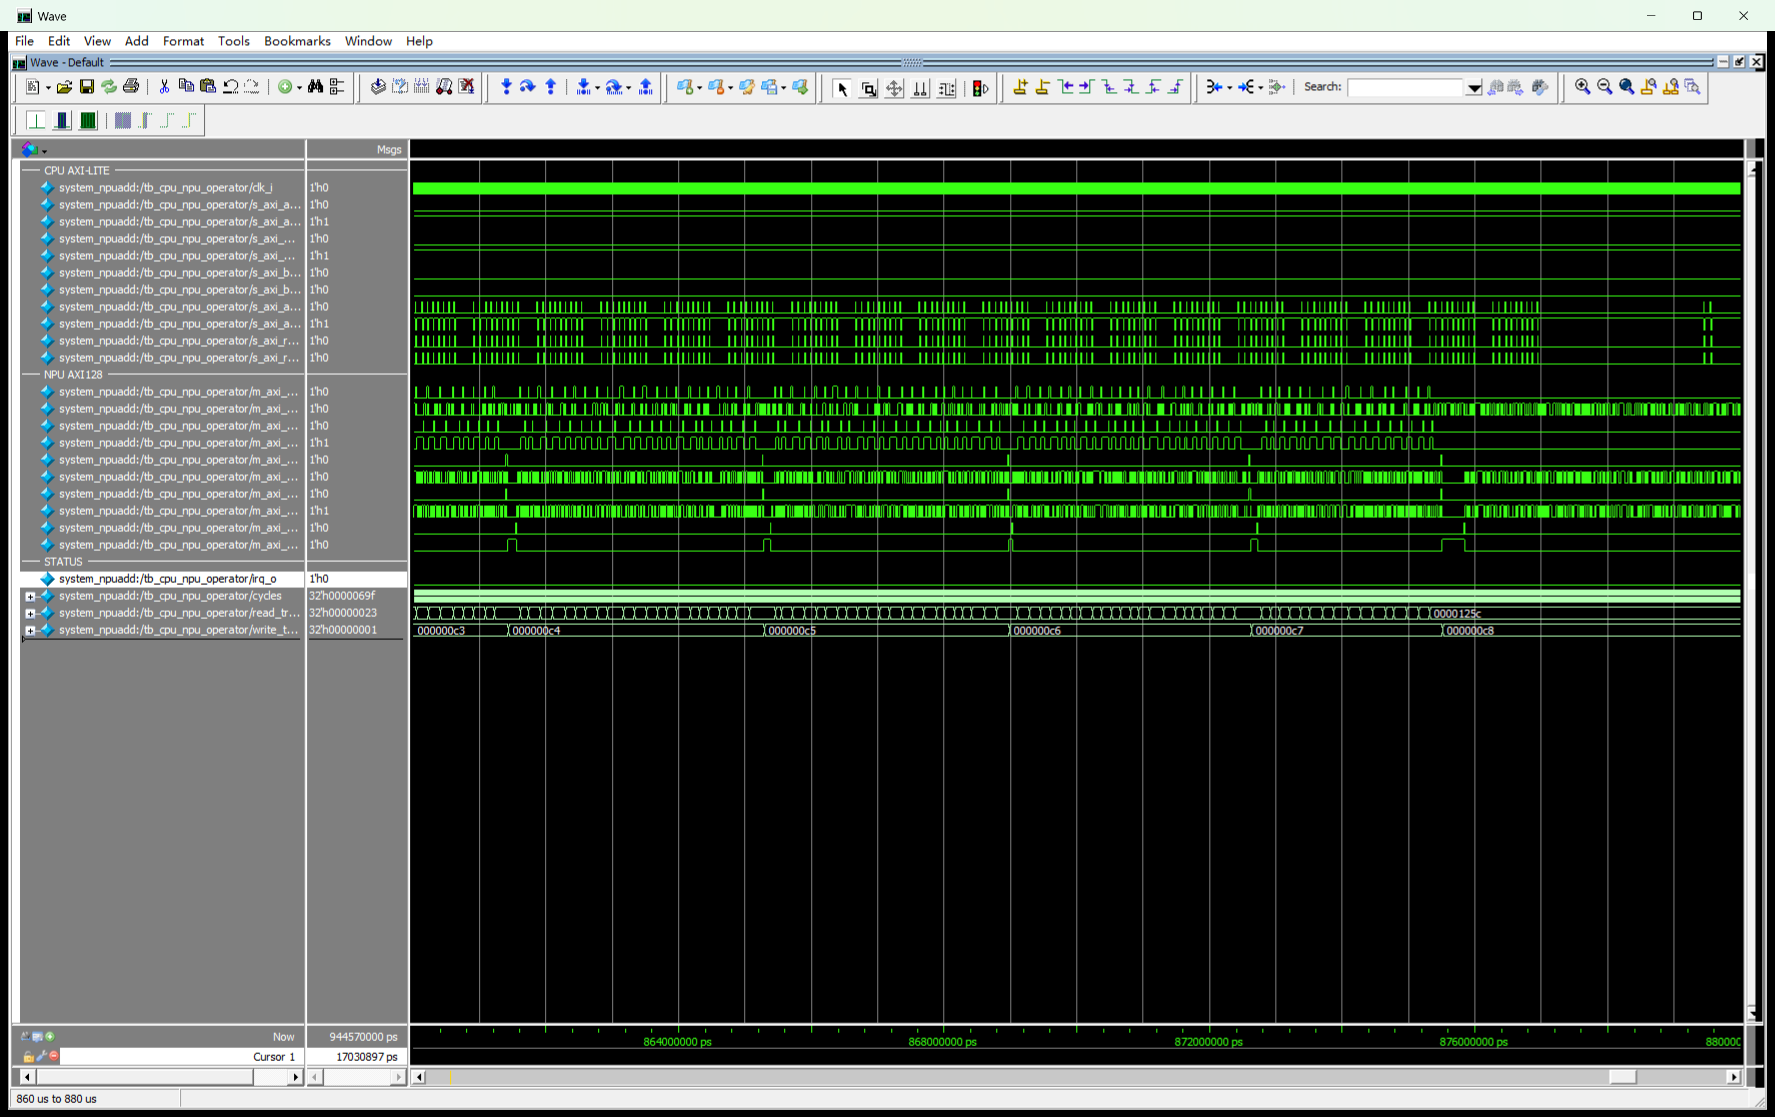
\includegraphics[width=0.8\linewidth]{../figure/system-interconnect-cpu-npu-complete-modelsim-original.png}
\caption{CPU到NPU尾部写响应、背压和事务计数收敛波形}
\label{fig:system-interconnect-cpu-npu-complete}
\end{figure}

\subsection{共享存储与地址译码}

Video共享DDR测试覆盖读写竞争、配额、释放、错误保持和背压传播；地址译码回归完成118项正常检查。对“错误目标选择”“过早接受W通道”和“请求与读响应对应错误”分别进行变异，三项均以非零诊断退出，说明地址译码及请求与响应对应关系的检查有效。

\begin{reporttable}
\begin{longtable}{@{}p{0.25\linewidth}p{0.31\linewidth}p{0.30\linewidth}p{0.08\linewidth}@{}}
\caption{系统互联与存储数字仿真结果}\\
\toprule
场景 & 覆盖内容 & 统计 & 结果 \\
\midrule
\endfirsthead
\caption[]{系统互联与存储数字仿真结果（续）}\\
\toprule
场景 & 覆盖内容 & 统计 & 结果 \\
\midrule
\endhead
\bottomrule
\endfoot
CPU到Video & 控制握手、三路写入、响应排空、完成和中断 & 6个正例、2个负例 & PASS \\
CPU到NPU & AXI-Lite配置、AXI128读写、轮询和中断完成 & 4个正例 & PASS \\
Video共享DDR & 读写竞争、配额、释放、错误保持和背压 & 共享DDR回归 & PASS \\
Video地址译码 & 目标选择、边界访问和请求与响应对应关系 & 118项正常、3项变异 & PASS \\
\end{longtable}
\end{reporttable}

上述结果来自使用本地存储模型的数字仿真，覆盖CPU外设控制、地址译码、读写握手、访问仲裁和错误响应。

